\chapter{Arhitektura i dizajn sustava}
	
		Arhitektura naše aplikacije može se intutivno podijeliti na prezentacijski, aplikacijski te podatkovni sloj. Njima redom odgovaraju idući podsustavi:
		\begin{itemize}
			\item 	Web aplikacija
			\item 	Web poslužitelj
			\item 	Baza podataka		
		\end{itemize}

		\begin{figure}[H]
			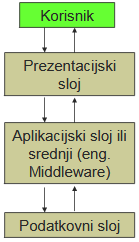
\includegraphics[scale=0.6]{slike/ArhitekturniPodsustavi.PNG}
			\centering
			\caption{Arhitektura sustava}
			\label{fig:arhitekturni_podsustavi}
		\end{figure}

		Kako bih se korisniku omogućilo korištenje naše aplikacije, korisnik na svojem uređaju (osobno računalo, laptop, mobitel ili tablet) mora koristiti \textit{web preglednik}, aplikaciju koja korištenjem stroja za vizualizaciju (u koji je uključen i interpreter JavaScript-a) omogućava
		pretvaranje koda naše web aplikacije (HTML, CSS i JavaScript) u vizualni multimedijski sadržaj.

		Za osnovnu komunikaciju s korisnikom koristi se \textit{web aplikacija}, program koji se pomoću HTTP (engl. \textit{Hyper Text Transfer Protocol}) protokola na zahtjev vraća korisnikovom web pregledniku. Web aplikacija služi kao sučelje između korisnika i poslovne logike aplikacije
		na web poslužitelju. Pomoću vizualnih komponenti korisniku se omogućava slanje HTTP zahtjeva na web poslužitelj te obrada i vizualizacija primljenih podataka u JSON (engl. \textit{JavaScript Object Notation}) formatu u ljudski razumljivom obliku.

		Primarni alat za komunikaciju s bazom podataka i za obradu poslovne logike je web poslužitelj kojem je omogućena komunikacija s web aplikacijom putem REST API (engl. \textit{Representational State Transfer Application Programming Interface}) tehnologije koja uvodi standardizirani način
		komunikacije s klijentom razmjenom JSON poruka. Na taj se način omogućava jasno određena i istovremeno fleksibilna razmjena podataka.

		Za izradu klijentske aplikacije izabrali smo jezik JavaScript zajedno s knjižnicom React koji omogućavaju jednostavnu i nativnu implementaciju arhitekture, zasnovane na događajima u klijentskom dijelu web aplikacije. Ovakav pristup omogućava dinamičko ažuriranje vizualnog prikaza na
		temelju korisničkih radnji i podataka, unesenih korisnikom. Kako bih se aplikacija mogla prikazati u korisnikovom web pregledniku, koristi se skupljač modula Webpack koji generira sve potrebne HTML, CSS i JavaScript datoteke koje se s poslužitelja šalju korisniku te se konačno prikazuju
		koristeći ugrađeni stroj za vizualizaciju web preglednika.

		Za opisivanje poslovne logike naše aplikacije odabrali smo programski jezik Java zajedno s radnim okvirom Spring Boot. Ovakav izbor tehnologija obrazložen je nativnom podrškom objektno usmjerenog pristupa programskim jezikom Java te jednostavnom implementacijom MVC 
		(engl. \textit{Model View Controller}) arhitekturnog modela u radnom okviru Spring Boot.

		MVC obrazac je stilistička varijacija arhitekture zasnovane na događajima koja se u našoj aplikaciji koristi kao alat za pojednostavljenje implementacije, testiranja i korištenja svih arhitekturnih podsustava. MVC obrazac dopušta paralelnu i neovisnu izradu tri komponente sustava
		na koje se intuitivno može podijeliti naša aplikacija:
		\begin{itemize}
			\item 	Model - Poslovna logika aplikacije koja definira i mijenja stanje koje aplikacija treba imati na temelju podataka iz kontrolera. 
			\item 	View - Vizualno sučelje ili korisnička strana aplikacije koja se koristi za vizualizaciju svih podataka unutar aplikacije, primarno dobivenih s web poslužitelja.
			\item 	Controller - Upravljački dio aplikacije koji komunikacijom s korisnikom kroz vizualni sloj ažurira stanje modela i/ili vizualnog stanja aplikacije.
		\end{itemize}

		\begin{figure}[H]
			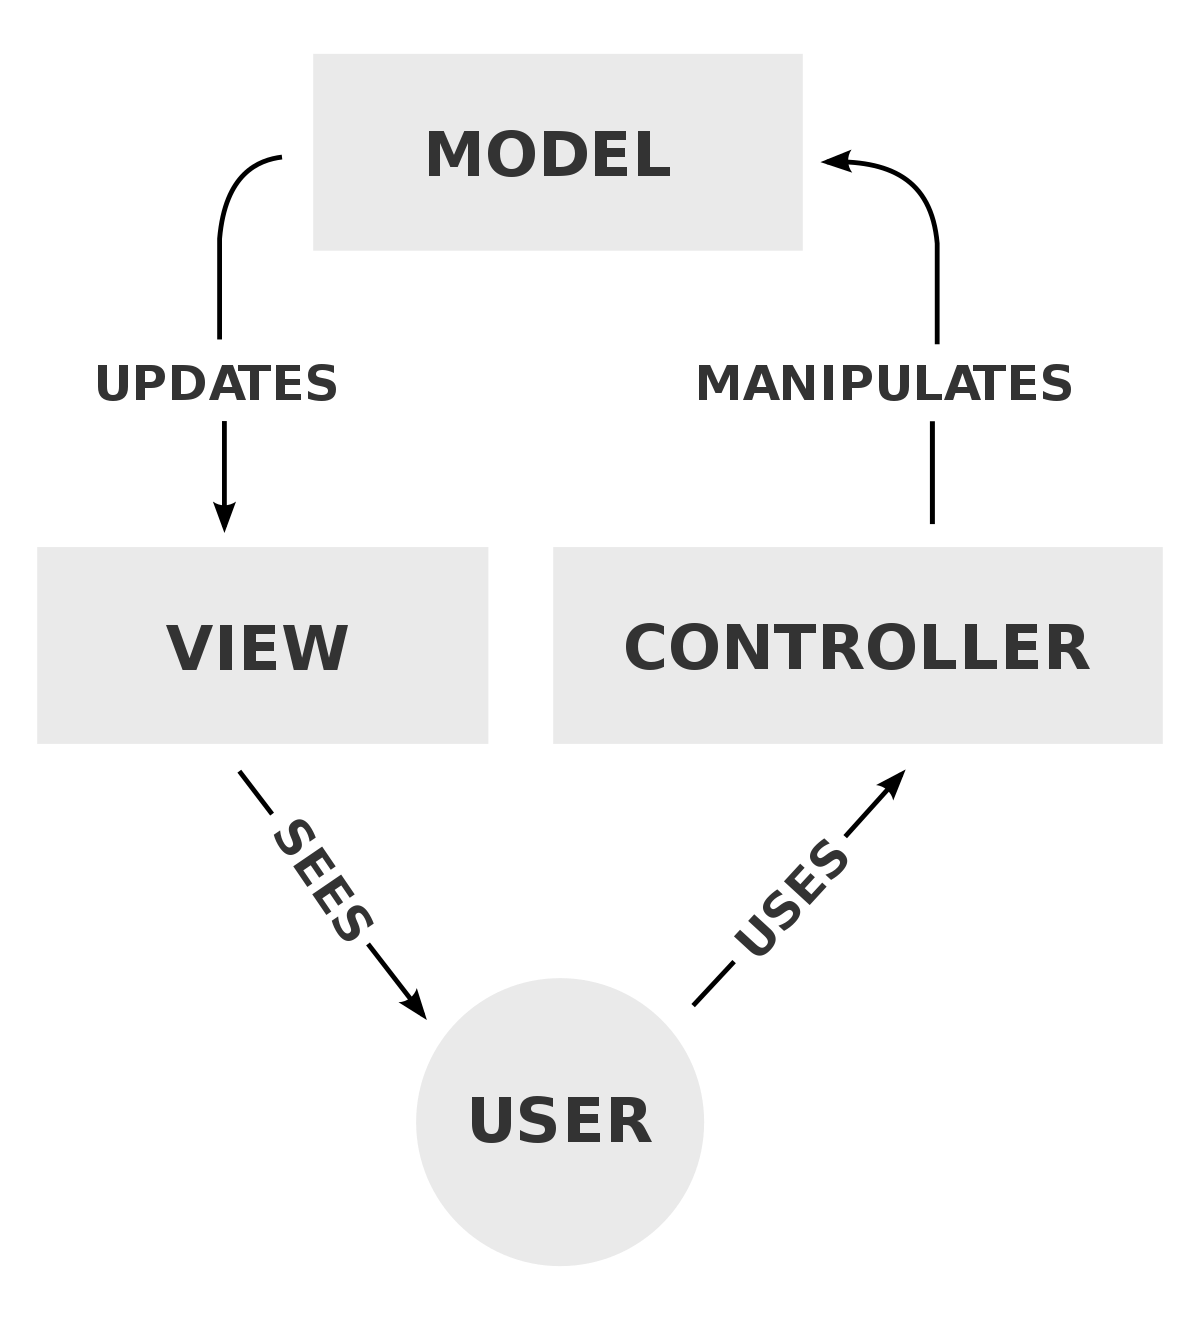
\includegraphics[scale=0.2]{slike/MVCObrazac.PNG}
			\centering
			\caption{MVC Obrazac}
			\label{fig:mvc_obrazac}
		\end{figure}

		\eject

				
		\section{Baza podataka}
			
			\textbf{\textit{dio 1. revizije}}\\
			
		\textit{Potrebno je opisati koju vrstu i implementaciju baze podataka ste odabrali, glavne komponente od kojih se sastoji i slično.}
		
			\subsection{Opis tablica}
			

				\textit{Svaku tablicu je potrebno opisati po zadanom predlošku. Lijevo se nalazi točno ime varijable u bazi podataka, u sredini se nalazi tip podataka, a desno se nalazi opis varijable. Svjetlozelenom bojom označite primarni ključ. Svjetlo plavom označite strani ključ}
				
				
				\begin{longtblr}[
					label=none,
					entry=none
					]{
						width = \textwidth,
						colspec={|X[6,l]|X[6, l]|X[20, l]|}, 
						rowhead = 1,
					} %definicija širine tablice, širine stupaca, poravnanje i broja redaka naslova tablice
					\hline \SetCell[c=3]{c}{\textbf{korisnik - ime tablice}}	 \\ \hline[3pt]
					\SetCell{LightGreen}IDKorisnik & INT	&  	Lorem ipsum dolor sit amet, consectetur adipiscing elit, sed do eiusmod  	\\ \hline
					korisnickoIme	& VARCHAR &   	\\ \hline 
					email & VARCHAR &   \\ \hline 
					ime & VARCHAR	&  		\\ \hline 
					\SetCell{LightBlue} primjer	& VARCHAR &   	\\ \hline 
				\end{longtblr}
				
				
			
			\subsection{Dijagram baze podataka}
				\textit{ U ovom potpoglavlju potrebno je umetnuti dijagram baze podataka. Primarni i strani ključevi moraju biti označeni, a tablice povezane. Bazu podataka je potrebno normalizirati. Podsjetite se kolegija "Baze podataka".}
			
			\eject
			
			
		\section{Dijagram razreda}
		
			\textit{Potrebno je priložiti dijagram razreda s pripadajućim opisom. Zbog preglednosti je moguće dijagram razlomiti na više njih, ali moraju biti grupirani prema sličnim razinama apstrakcije i srodnim funkcionalnostima.}\\
			
			\textbf{\textit{dio 1. revizije}}\\
			
			\textit{Prilikom prve predaje projekta, potrebno je priložiti potpuno razrađen dijagram razreda vezan uz \textbf{generičku funkcionalnost} sustava. Ostale funkcionalnosti trebaju biti idejno razrađene u dijagramu sa sljedećim komponentama: nazivi razreda, nazivi metoda i vrste pristupa metodama (npr. javni, zaštićeni), nazivi atributa razreda, veze i odnosi između razreda.}\\
			
			\textbf{\textit{dio 2. revizije}}\\			
			
			\textit{Prilikom druge predaje projekta dijagram razreda i opisi moraju odgovarati stvarnom stanju implementacije}
			
			
			
			\eject
		
		\section{Dijagram stanja}
			
			
			\textbf{\textit{dio 2. revizije}}\\
			
			\textit{Potrebno je priložiti dijagram stanja i opisati ga. Dovoljan je jedan dijagram stanja koji prikazuje \textbf{značajan dio funkcionalnosti} sustava. Na primjer, stanja korisničkog sučelja i tijek korištenja neke ključne funkcionalnosti jesu značajan dio sustava, a registracija i prijava nisu. }
			
			
			\eject 
		
		\section{Dijagram aktivnosti}
			
			\textbf{\textit{dio 2. revizije}}\\
			
			 \textit{Potrebno je priložiti dijagram aktivnosti s pripadajućim opisom. Dijagram aktivnosti treba prikazivati značajan dio sustava.}
			
			\eject
		\section{Dijagram komponenti}
		
			\textbf{\textit{dio 2. revizije}}\\
		
			 \textit{Potrebno je priložiti dijagram komponenti s pripadajućim opisom. Dijagram komponenti treba prikazivati strukturu cijele aplikacije.}